
% Inherit from the specified cell style.

% Default to the notebook output style

    


% Inherit from the specified cell style.




    
\documentclass[letter]{article}

    
    
% \usepackage{stix}
% \usepackage[scr]{rsfso}
% \usepackage{bm}

\usepackage[T1]{fontenc}
% Nicer default font than Computer Modern for most use cases
\usepackage{palatino}

% Basic figure setup, for now with no caption control since it's done
% automatically by Pandoc (which extracts ![](path) syntax from Markdown).
\usepackage{graphicx}
% We will generate all images so they have a width \maxwidth. This means
% that they will get their normal width if they fit onto the page, but
% are scaled down if they would overflow the margins.
\makeatletter
\def\maxwidth{\ifdim\Gin@nat@width>\linewidth\linewidth
\else\Gin@nat@width\fi}
\makeatother
\let\Oldincludegraphics\includegraphics
% Set max figure width to be 80% of text width, for now hardcoded.
\renewcommand{\includegraphics}[1]{\Oldincludegraphics[width=.8\maxwidth]{#1}}
% Ensure that by default, figures have no caption (until we provide a
% proper Figure object with a Caption API and a way to capture that
% in the conversion process - todo).
% \usepackage{caption}
% \DeclareCaptionLabelFormat{nolabel}{}
% \captionsetup{labelformat=nolabel}

\usepackage{adjustbox} % Used to constrain images to a maximum size 
\usepackage{xcolor} % Allow colors to be defined
\usepackage{enumerate} % Needed for markdown enumerations to work
\usepackage{geometry} % Used to adjust the document margins
\usepackage{amsmath} % Equations
\usepackage{amssymb} % Equations
\usepackage{textcomp} % defines textquotesingle
% Hack from http://tex.stackexchange.com/a/47451/13684:
\AtBeginDocument{%
    \def\PYZsq{\textquotesingle}% Upright quotes in Pygmentized code
}
\usepackage{upquote} % Upright quotes for verbatim code
\usepackage{eurosym} % defines \euro
\usepackage[mathletters]{ucs} % Extended unicode (utf-8) support
\usepackage[utf8x]{inputenc} % Allow utf-8 characters in the tex document
\usepackage{fancyvrb} % verbatim replacement that allows latex
\usepackage{grffile} % extends the file name processing of package graphics 
                     % to support a larger range 
% The hyperref package gives us a pdf with properly built
% internal navigation ('pdf bookmarks' for the table of contents,
% internal cross-reference links, web links for URLs, etc.)
\usepackage{hyperref}
\usepackage{longtable} % longtable support required by pandoc >1.10
\usepackage{booktabs}  % table support for pandoc > 1.12.2
\usepackage[normalem]{ulem} % ulem is needed to support strikethroughs (\sout)
                            % normalem makes italics be italics, not underlines



    
    
    
    % Colors for the hyperref package
    \definecolor{urlcolor}{rgb}{0,.145,.698}
    \definecolor{linkcolor}{rgb}{.71,0.21,0.01}
    \definecolor{citecolor}{rgb}{.12,.54,.11}

    % ANSI colors
    \definecolor{ansi-black}{HTML}{3E424D}
    \definecolor{ansi-black-intense}{HTML}{282C36}
    \definecolor{ansi-red}{HTML}{E75C58}
    \definecolor{ansi-red-intense}{HTML}{B22B31}
    \definecolor{ansi-green}{HTML}{00A250}
    \definecolor{ansi-green-intense}{HTML}{007427}
    \definecolor{ansi-yellow}{HTML}{DDB62B}
    \definecolor{ansi-yellow-intense}{HTML}{B27D12}
    \definecolor{ansi-blue}{HTML}{208FFB}
    \definecolor{ansi-blue-intense}{HTML}{0065CA}
    \definecolor{ansi-magenta}{HTML}{D160C4}
    \definecolor{ansi-magenta-intense}{HTML}{A03196}
    \definecolor{ansi-cyan}{HTML}{60C6C8}
    \definecolor{ansi-cyan-intense}{HTML}{258F8F}
    \definecolor{ansi-white}{HTML}{C5C1B4}
    \definecolor{ansi-white-intense}{HTML}{A1A6B2}

    % commands and environments needed by pandoc snippets
    % extracted from the output of `pandoc -s`
    \providecommand{\tightlist}{%
      \setlength{\itemsep}{0pt}\setlength{\parskip}{0pt}}
    \DefineVerbatimEnvironment{Highlighting}{Verbatim}{commandchars=\\\{\}}
    % Add ',fontsize=\small' for more characters per line
    \newenvironment{Shaded}{}{}
    \newcommand{\KeywordTok}[1]{\textcolor[rgb]{0.00,0.44,0.13}{\textbf{{#1}}}}
    \newcommand{\DataTypeTok}[1]{\textcolor[rgb]{0.56,0.13,0.00}{{#1}}}
    \newcommand{\DecValTok}[1]{\textcolor[rgb]{0.25,0.63,0.44}{{#1}}}
    \newcommand{\BaseNTok}[1]{\textcolor[rgb]{0.25,0.63,0.44}{{#1}}}
    \newcommand{\FloatTok}[1]{\textcolor[rgb]{0.25,0.63,0.44}{{#1}}}
    \newcommand{\CharTok}[1]{\textcolor[rgb]{0.25,0.44,0.63}{{#1}}}
    \newcommand{\StringTok}[1]{\textcolor[rgb]{0.25,0.44,0.63}{{#1}}}
    \newcommand{\CommentTok}[1]{\textcolor[rgb]{0.38,0.63,0.69}{\textit{{#1}}}}
    \newcommand{\OtherTok}[1]{\textcolor[rgb]{0.00,0.44,0.13}{{#1}}}
    \newcommand{\AlertTok}[1]{\textcolor[rgb]{1.00,0.00,0.00}{\textbf{{#1}}}}
    \newcommand{\FunctionTok}[1]{\textcolor[rgb]{0.02,0.16,0.49}{{#1}}}
    \newcommand{\RegionMarkerTok}[1]{{#1}}
    \newcommand{\ErrorTok}[1]{\textcolor[rgb]{1.00,0.00,0.00}{\textbf{{#1}}}}
    \newcommand{\NormalTok}[1]{{#1}}
    
    % Additional commands for more recent versions of Pandoc
    \newcommand{\ConstantTok}[1]{\textcolor[rgb]{0.53,0.00,0.00}{{#1}}}
    \newcommand{\SpecialCharTok}[1]{\textcolor[rgb]{0.25,0.44,0.63}{{#1}}}
    \newcommand{\VerbatimStringTok}[1]{\textcolor[rgb]{0.25,0.44,0.63}{{#1}}}
    \newcommand{\SpecialStringTok}[1]{\textcolor[rgb]{0.73,0.40,0.53}{{#1}}}
    \newcommand{\ImportTok}[1]{{#1}}
    \newcommand{\DocumentationTok}[1]{\textcolor[rgb]{0.73,0.13,0.13}{\textit{{#1}}}}
    \newcommand{\AnnotationTok}[1]{\textcolor[rgb]{0.38,0.63,0.69}{\textbf{\textit{{#1}}}}}
    \newcommand{\CommentVarTok}[1]{\textcolor[rgb]{0.38,0.63,0.69}{\textbf{\textit{{#1}}}}}
    \newcommand{\VariableTok}[1]{\textcolor[rgb]{0.10,0.09,0.49}{{#1}}}
    \newcommand{\ControlFlowTok}[1]{\textcolor[rgb]{0.00,0.44,0.13}{\textbf{{#1}}}}
    \newcommand{\OperatorTok}[1]{\textcolor[rgb]{0.40,0.40,0.40}{{#1}}}
    \newcommand{\BuiltInTok}[1]{{#1}}
    \newcommand{\ExtensionTok}[1]{{#1}}
    \newcommand{\PreprocessorTok}[1]{\textcolor[rgb]{0.74,0.48,0.00}{{#1}}}
    \newcommand{\AttributeTok}[1]{\textcolor[rgb]{0.49,0.56,0.16}{{#1}}}
    \newcommand{\InformationTok}[1]{\textcolor[rgb]{0.38,0.63,0.69}{\textbf{\textit{{#1}}}}}
    \newcommand{\WarningTok}[1]{\textcolor[rgb]{0.38,0.63,0.69}{\textbf{\textit{{#1}}}}}
    
    
    % Define a nice break command that doesn't care if a line doesn't already
    % exist.
    \def\br{\hspace*{\fill} \\* }
    % Math Jax compatability definitions
    \def\gt{>}
    \def\lt{<}
    % Document parameters
    \title{TemperatureImputations}
    
    \author{Maxime Rischard}
    

    % Pygments definitions
    
\makeatletter
\def\PY@reset{\let\PY@it=\relax \let\PY@bf=\relax%
    \let\PY@ul=\relax \let\PY@tc=\relax%
    \let\PY@bc=\relax \let\PY@ff=\relax}
\def\PY@tok#1{\csname PY@tok@#1\endcsname}
\def\PY@toks#1+{\ifx\relax#1\empty\else%
    \PY@tok{#1}\expandafter\PY@toks\fi}
\def\PY@do#1{\PY@bc{\PY@tc{\PY@ul{%
    \PY@it{\PY@bf{\PY@ff{#1}}}}}}}
\def\PY#1#2{\PY@reset\PY@toks#1+\relax+\PY@do{#2}}

\expandafter\def\csname PY@tok@ch\endcsname{\let\PY@it=\textit\def\PY@tc##1{\textcolor[rgb]{0.25,0.50,0.50}{##1}}}
\expandafter\def\csname PY@tok@cpf\endcsname{\let\PY@it=\textit\def\PY@tc##1{\textcolor[rgb]{0.25,0.50,0.50}{##1}}}
\expandafter\def\csname PY@tok@s2\endcsname{\def\PY@tc##1{\textcolor[rgb]{0.73,0.13,0.13}{##1}}}
\expandafter\def\csname PY@tok@kr\endcsname{\let\PY@bf=\textbf\def\PY@tc##1{\textcolor[rgb]{0.00,0.50,0.00}{##1}}}
\expandafter\def\csname PY@tok@c1\endcsname{\let\PY@it=\textit\def\PY@tc##1{\textcolor[rgb]{0.25,0.50,0.50}{##1}}}
\expandafter\def\csname PY@tok@ni\endcsname{\let\PY@bf=\textbf\def\PY@tc##1{\textcolor[rgb]{0.60,0.60,0.60}{##1}}}
\expandafter\def\csname PY@tok@sh\endcsname{\def\PY@tc##1{\textcolor[rgb]{0.73,0.13,0.13}{##1}}}
\expandafter\def\csname PY@tok@na\endcsname{\def\PY@tc##1{\textcolor[rgb]{0.49,0.56,0.16}{##1}}}
\expandafter\def\csname PY@tok@w\endcsname{\def\PY@tc##1{\textcolor[rgb]{0.73,0.73,0.73}{##1}}}
\expandafter\def\csname PY@tok@o\endcsname{\def\PY@tc##1{\textcolor[rgb]{0.40,0.40,0.40}{##1}}}
\expandafter\def\csname PY@tok@nc\endcsname{\let\PY@bf=\textbf\def\PY@tc##1{\textcolor[rgb]{0.00,0.00,1.00}{##1}}}
\expandafter\def\csname PY@tok@nd\endcsname{\def\PY@tc##1{\textcolor[rgb]{0.67,0.13,1.00}{##1}}}
\expandafter\def\csname PY@tok@gr\endcsname{\def\PY@tc##1{\textcolor[rgb]{1.00,0.00,0.00}{##1}}}
\expandafter\def\csname PY@tok@ss\endcsname{\def\PY@tc##1{\textcolor[rgb]{0.10,0.09,0.49}{##1}}}
\expandafter\def\csname PY@tok@gh\endcsname{\let\PY@bf=\textbf\def\PY@tc##1{\textcolor[rgb]{0.00,0.00,0.50}{##1}}}
\expandafter\def\csname PY@tok@bp\endcsname{\def\PY@tc##1{\textcolor[rgb]{0.00,0.50,0.00}{##1}}}
\expandafter\def\csname PY@tok@sb\endcsname{\def\PY@tc##1{\textcolor[rgb]{0.73,0.13,0.13}{##1}}}
\expandafter\def\csname PY@tok@go\endcsname{\def\PY@tc##1{\textcolor[rgb]{0.53,0.53,0.53}{##1}}}
\expandafter\def\csname PY@tok@nv\endcsname{\def\PY@tc##1{\textcolor[rgb]{0.10,0.09,0.49}{##1}}}
\expandafter\def\csname PY@tok@gp\endcsname{\let\PY@bf=\textbf\def\PY@tc##1{\textcolor[rgb]{0.00,0.00,0.50}{##1}}}
\expandafter\def\csname PY@tok@c\endcsname{\let\PY@it=\textit\def\PY@tc##1{\textcolor[rgb]{0.25,0.50,0.50}{##1}}}
\expandafter\def\csname PY@tok@k\endcsname{\let\PY@bf=\textbf\def\PY@tc##1{\textcolor[rgb]{0.00,0.50,0.00}{##1}}}
\expandafter\def\csname PY@tok@gi\endcsname{\def\PY@tc##1{\textcolor[rgb]{0.00,0.63,0.00}{##1}}}
\expandafter\def\csname PY@tok@gu\endcsname{\let\PY@bf=\textbf\def\PY@tc##1{\textcolor[rgb]{0.50,0.00,0.50}{##1}}}
\expandafter\def\csname PY@tok@kt\endcsname{\def\PY@tc##1{\textcolor[rgb]{0.69,0.00,0.25}{##1}}}
\expandafter\def\csname PY@tok@vc\endcsname{\def\PY@tc##1{\textcolor[rgb]{0.10,0.09,0.49}{##1}}}
\expandafter\def\csname PY@tok@cs\endcsname{\let\PY@it=\textit\def\PY@tc##1{\textcolor[rgb]{0.25,0.50,0.50}{##1}}}
\expandafter\def\csname PY@tok@nt\endcsname{\let\PY@bf=\textbf\def\PY@tc##1{\textcolor[rgb]{0.00,0.50,0.00}{##1}}}
\expandafter\def\csname PY@tok@m\endcsname{\def\PY@tc##1{\textcolor[rgb]{0.40,0.40,0.40}{##1}}}
\expandafter\def\csname PY@tok@kp\endcsname{\def\PY@tc##1{\textcolor[rgb]{0.00,0.50,0.00}{##1}}}
\expandafter\def\csname PY@tok@cm\endcsname{\let\PY@it=\textit\def\PY@tc##1{\textcolor[rgb]{0.25,0.50,0.50}{##1}}}
\expandafter\def\csname PY@tok@nb\endcsname{\def\PY@tc##1{\textcolor[rgb]{0.00,0.50,0.00}{##1}}}
\expandafter\def\csname PY@tok@sc\endcsname{\def\PY@tc##1{\textcolor[rgb]{0.73,0.13,0.13}{##1}}}
\expandafter\def\csname PY@tok@kn\endcsname{\let\PY@bf=\textbf\def\PY@tc##1{\textcolor[rgb]{0.00,0.50,0.00}{##1}}}
\expandafter\def\csname PY@tok@nl\endcsname{\def\PY@tc##1{\textcolor[rgb]{0.63,0.63,0.00}{##1}}}
\expandafter\def\csname PY@tok@vg\endcsname{\def\PY@tc##1{\textcolor[rgb]{0.10,0.09,0.49}{##1}}}
\expandafter\def\csname PY@tok@sd\endcsname{\let\PY@it=\textit\def\PY@tc##1{\textcolor[rgb]{0.73,0.13,0.13}{##1}}}
\expandafter\def\csname PY@tok@mo\endcsname{\def\PY@tc##1{\textcolor[rgb]{0.40,0.40,0.40}{##1}}}
\expandafter\def\csname PY@tok@no\endcsname{\def\PY@tc##1{\textcolor[rgb]{0.53,0.00,0.00}{##1}}}
\expandafter\def\csname PY@tok@kc\endcsname{\let\PY@bf=\textbf\def\PY@tc##1{\textcolor[rgb]{0.00,0.50,0.00}{##1}}}
\expandafter\def\csname PY@tok@mi\endcsname{\def\PY@tc##1{\textcolor[rgb]{0.40,0.40,0.40}{##1}}}
\expandafter\def\csname PY@tok@mb\endcsname{\def\PY@tc##1{\textcolor[rgb]{0.40,0.40,0.40}{##1}}}
\expandafter\def\csname PY@tok@s\endcsname{\def\PY@tc##1{\textcolor[rgb]{0.73,0.13,0.13}{##1}}}
\expandafter\def\csname PY@tok@sr\endcsname{\def\PY@tc##1{\textcolor[rgb]{0.73,0.40,0.53}{##1}}}
\expandafter\def\csname PY@tok@mf\endcsname{\def\PY@tc##1{\textcolor[rgb]{0.40,0.40,0.40}{##1}}}
\expandafter\def\csname PY@tok@ge\endcsname{\let\PY@it=\textit}
\expandafter\def\csname PY@tok@cp\endcsname{\def\PY@tc##1{\textcolor[rgb]{0.74,0.48,0.00}{##1}}}
\expandafter\def\csname PY@tok@ow\endcsname{\let\PY@bf=\textbf\def\PY@tc##1{\textcolor[rgb]{0.67,0.13,1.00}{##1}}}
\expandafter\def\csname PY@tok@gs\endcsname{\let\PY@bf=\textbf}
\expandafter\def\csname PY@tok@il\endcsname{\def\PY@tc##1{\textcolor[rgb]{0.40,0.40,0.40}{##1}}}
\expandafter\def\csname PY@tok@kd\endcsname{\let\PY@bf=\textbf\def\PY@tc##1{\textcolor[rgb]{0.00,0.50,0.00}{##1}}}
\expandafter\def\csname PY@tok@se\endcsname{\let\PY@bf=\textbf\def\PY@tc##1{\textcolor[rgb]{0.73,0.40,0.13}{##1}}}
\expandafter\def\csname PY@tok@sx\endcsname{\def\PY@tc##1{\textcolor[rgb]{0.00,0.50,0.00}{##1}}}
\expandafter\def\csname PY@tok@nn\endcsname{\let\PY@bf=\textbf\def\PY@tc##1{\textcolor[rgb]{0.00,0.00,1.00}{##1}}}
\expandafter\def\csname PY@tok@gd\endcsname{\def\PY@tc##1{\textcolor[rgb]{0.63,0.00,0.00}{##1}}}
\expandafter\def\csname PY@tok@ne\endcsname{\let\PY@bf=\textbf\def\PY@tc##1{\textcolor[rgb]{0.82,0.25,0.23}{##1}}}
\expandafter\def\csname PY@tok@gt\endcsname{\def\PY@tc##1{\textcolor[rgb]{0.00,0.27,0.87}{##1}}}
\expandafter\def\csname PY@tok@nf\endcsname{\def\PY@tc##1{\textcolor[rgb]{0.00,0.00,1.00}{##1}}}
\expandafter\def\csname PY@tok@err\endcsname{\def\PY@bc##1{\setlength{\fboxsep}{0pt}\fcolorbox[rgb]{1.00,0.00,0.00}{1,1,1}{\strut ##1}}}
\expandafter\def\csname PY@tok@vi\endcsname{\def\PY@tc##1{\textcolor[rgb]{0.10,0.09,0.49}{##1}}}
\expandafter\def\csname PY@tok@s1\endcsname{\def\PY@tc##1{\textcolor[rgb]{0.73,0.13,0.13}{##1}}}
\expandafter\def\csname PY@tok@mh\endcsname{\def\PY@tc##1{\textcolor[rgb]{0.40,0.40,0.40}{##1}}}
\expandafter\def\csname PY@tok@si\endcsname{\let\PY@bf=\textbf\def\PY@tc##1{\textcolor[rgb]{0.73,0.40,0.53}{##1}}}

\def\PYZbs{\char`\\}
\def\PYZus{\char`\_}
\def\PYZob{\char`\{}
\def\PYZcb{\char`\}}
\def\PYZca{\char`\^}
\def\PYZam{\char`\&}
\def\PYZlt{\char`\<}
\def\PYZgt{\char`\>}
\def\PYZsh{\char`\#}
\def\PYZpc{\char`\%}
\def\PYZdl{\char`\$}
\def\PYZhy{\char`\-}
\def\PYZsq{\char`\'}
\def\PYZdq{\char`\"}
\def\PYZti{\char`\~}
% for compatibility with earlier versions
\def\PYZat{@}
\def\PYZlb{[}
\def\PYZrb{]}
\makeatother


    % Exact colors from NB
    \definecolor{incolor}{rgb}{0.0, 0.0, 0.5}
    \definecolor{outcolor}{rgb}{0.545, 0.0, 0.0}


    \newcommand{\genericdel}[3]{%
      \left#1#3\right#2
    }
    \newcommand{\del}[1]{\genericdel(){#1}}
    \newcommand{\sbr}[1]{\genericdel[]{#1}}
    \newcommand{\cbr}[1]{\genericdel\{\}{#1}}
    \DeclareMathOperator*{\argmin}{arg\,min}
    \DeclareMathOperator*{\argmax}{arg\,max}
    \let\Pr\relax
    \DeclareMathOperator{\Pr}{\mathbb{P}}
    \DeclareMathOperator{\E}{\mathbb{E}}
    \DeclareMathOperator{\V}{\mathbb{V}}
    \DeclareMathOperator{\cov}{{cov}}
    \DeclareMathOperator{\var}{{var}}
    \DeclareMathOperator{\Ind}{\mathbb{I}}
    \DeclareMathOperator*{\sgn}{{sgn}}
   % \DeclareMathOperator{\invchi}{\mathrm{Inv-\chi}^2}}
   \DeclareMathOperator{\normal}{\mathcal{N}}
   \DeclareMathOperator{\unif}{Uniform}
   \DeclareMathOperator{\GP}{\mathcal{GP}}
   \newcommand{\Tn}{\mathrm{T}_{n}}
   \newcommand{\Tx}{\mathrm{T}_{x}}
   \newcommand{\station}[1]{\mathrm{station}\sbr{#1}}
   \newcommand{\xvec}{\mathbf{x}}
   \newcommand{\indep}{\perp}
   \newcommand{\iid}{iid}
   \newcommand{\trans}{^{\intercal}}
   \newcommand{\sigmaf}{\sigma_{\mathrm{GP}}}
   \newcommand{\sigman}{\sigma_{\epsilon}}
   \newcommand{\degreeC}{^\circ \mathrm{C}}
   \newcommand{\miss}{\mathrm{miss}}
   \newcommand{\obs}{\mathrm{obs}}
   \DeclareMathOperator{\softmax}{smoothmax}
   \DeclareMathOperator{\softmin}{smoothmin}

	\providecommand{\tightlist}{%
  	  \setlength{\itemsep}{0pt}\setlength{\parskip}{0pt}}


    
    % Prevent overflowing lines due to hard-to-break entities
    \sloppy 
    % Setup hyperref package
    \hypersetup{
      breaklinks=true,  % so long urls are correctly broken across lines
      colorlinks=true,
      urlcolor=urlcolor,
      linkcolor=linkcolor,
      citecolor=citecolor,
      }
    % Slightly bigger margins than the latex defaults
    
    \geometry{verbose,tmargin=1in,bmargin=1in,lmargin=1in,rmargin=1in}
    
    

    \begin{document}
    
    
    
    \maketitle
    
    
	\tableofcontents


    







    	\section{Introduction}\label{introduction}

\begin{itemize}
\tightlist
\item
  explain the problem we're trying to solve
\end{itemize}

\subsection{bias in recorded daily minima and maxima induced by time of
measurement}\label{bias-in-recorded-daily-minima-and-maxima-induced-by-time-of-measurement}

\begin{itemize}
\tightlist
\item
  explain
\item
  demonstrate using hourly temperatures from one station: reduce to
  daily min and max and show difference as a function of measurement
  hour
\end{itemize}
    


    	We illustrate the measurement bias in daily maxima and minima with ten
days of hourly temperature measurements from the Waterloo Municipal
Airport station in Iowa. Ideally, \(\Tx\) measurements should capture
the peak of each diurnal cycle, and \(\Tn\) its trough. In Figure X,
those ideal measurements are indicated by the red and blue triangles
respectively. The actual measurements are obtained by dividing the data
into 24 hour measurement windows, and extracting the minimum and
maximum. For each window, we plot these extrema with a red and blue
horizontal line.

On most days, the ideal measurement and the actual measurement coincide:
the triangle is on that day's line. But there are also several misses.
The most blatant example occurs on April 3rd, where the peak of the
diurnal cycle is \{\{apr3\_realmax\}\}°C and occurs at 21:00 UTC.
However, because the previous day was much warmer, the day's \(\Tx\)
record of \{\{apr3\_measured\}\}°C is reached immediately after the
previous day's measurement. The measured \(\Tx\) therefore overestimates
the diurnal cycle's peak by
\{\{round(apr3\_measured-apr3\_realmax,1)\}\}°C.
    



    			
    \begin{figure}[tbh]
    \begin{center}
    \adjustimage{max size={0.8\linewidth}{0.5\paperheight}}{TemperatureImputations_files/TemperatureImputations_6_0.png}
    \end{center}
    { \hspace*{\fill} \\}
	\end{figure}
    
    		

    			
    \begin{figure}[tbh]
    \begin{center}
    \adjustimage{max size={0.8\linewidth}{0.5\paperheight}}{TemperatureImputations_files/TemperatureImputations_7_0.png}
    \end{center}
    { \hspace*{\fill} \\}
	\end{figure}
    
    		

    			
    \begin{figure}[tbh]
    \begin{center}
    \adjustimage{max size={0.8\linewidth}{0.5\paperheight}}{TemperatureImputations_files/TemperatureImputations_8_0.png}
    \end{center}
    { \hspace*{\fill} \\}
	\end{figure}
    
    		
    	This subtle bias in the daily records can in turn bias long-term summary
statistics that are of climatological interest. A measure as simple as
the average daily maximum temperature for an entire year (2015)
increases by over 1°C if the measurements are made at the warmest time
of day 21:00 UTC rather than 14:00 UTC (see Figure X). Conversely, the
average \(\Tn\) is colder by over 1°C if \(\Tn\) is measured at 10:00
UTC (the coldest time of day on average) rather than 17:00 UTC.

A climatologist studying weather variability might be interested in
summary statistics such as the average absolute change in the daily
temperature maxima and minima from one day to the next. The answer to
that question too depends on the time of day at which the temperatures
are recorded. Collecting the measurements at the hottest time of day
means that the peaks on a warm day gets recorded twice, erasing the
diurnal peaks of the following colder day, and hence the variability
gets underestimated. We can see this in Figure X, where the respective
variability estimates drop if the maxima get measured at the warmest
time, or if the minima get measured at the coldest time.
    


    	\subsection{Proposed solution}\label{proposed-solution}

We have seen that the daily maxima and minima do not faithfully record
each diurnal cycle's peak and trough. The peaks on a relatively cold day
can get overwritten by temperatures at either end of the measurement
window that properly belong to the previous or the next diurnal cycle.
Troughs on relatively warm days can be similarly overwritten. Our goal
is to undo this damage, and recover estimates of summary statistics,
such as the average daily maximum temperature, that do not suffer from
the consequent bias. We need to address the erasure of information
caused by the measurement mechanism, and therefore view this as a
missing data problem.

Taking the missing data perspective, we seek to impute the hourly
temperatures that have been replaced by a maximum and minimum over a 24
hour period. To do so, we use information from two sources: the recorded
daily temperature extremes at the station of interest, and also hourly
temperatures recorded at nearby meteorological stations. These hourly
measurements are considered less reliable by climatologists, as they
aren't as carefully documented, calibrated, and situated. The
meterological stations are often in locations (like airports) where
human activity will affect temperatures. Therefore, summary statistics
extracted directly from those measurements would not be directly usable
for climatology, as they could suffer from systematic bias. However,
even if miscalibrated, the meterological data do contain valuable
information about the hourly changes in temperatures on any given day.
We therefore use them to inform the shape of the imputed temperature
time-series at our location of interest, while we use the recorded
temperature extrema to calibrate and constrain them.
    


    	\section{First Spatiotemporal Model}\label{first-spatiotemporal-model}

To model measured temperatures at various locations and times, we use a
spatio-temporal Gaussian process model. In its simplest form, we believe
that temperatures from stations that are near each other are more
correlated than distant stations, and that those correlations should
also decay in time. In the spatial statistics literature, squared
exponential covariance functions are commonly used to model correlations
decaying as a function of distance. Ignoring the time dimension, we
would model the simultaneous temperatures throughout a region as a
Gaussian process, with the covariance of two locations \(\xvec\) and
\(\xvec'\)

\begin{equation}
    \cov\del{T(\xvec), T(\xvec') \mid t} = k_{space}(\xvec, \xvec') = \sigmaf^2 \exp\del{-\frac{\del{\xvec-\xvec'}\trans\del{\xvec-\xvec'}}{2\ell_x^2}}\,.
\end{equation}

Similarly, ignoring the spatial dimension, the time series of
temperatures at a single location can be modeled as a Gaussian process
with covariance between two moments \(t\) and \(t'\)

\begin{equation}
\cov\del{T(t), T(t') \mid \xvec} = k_{time}(t, t') = \sigmaf^2 \exp\del{-\frac{\del{t-t'}^2}{2\ell_t^2}}\,.
\end{equation}

We then combine the spatial and temporal model by multiplying the
covariance functions

\begin{equation}
k_{st}(\xvec,\xvec',t,t') = k_{time}(t,t') \cdot k_{space}(\xvec, \xvec')\,.
\end{equation}

This gives us the covariance of the Gaussian process underlying the full
spatio-temporal model of temperatures. To complete the model
specification, we add a mean temperature for each station
\(\mu_{\station{i}}\), and iid measurement noise \(\epsilon_i\).

\begin{align}
    T_i &= \mu_{\station{i}} + f(\xvec_i, t_i) + \epsilon_i\\
    f(\xvec_i, t_i) &\sim \GP\del{0, k_{st}(\xvec,\xvec',t,t')}\\
    \epsilon_i &\overset{\iid}{\sim} \normal\del{0,\sigman^2}\\
\end{align}
    


    	\section{Fitting the spatiotemporal
model}\label{fitting-the-spatiotemporal-model}

Software is readily available in many programming languages for fitting
Gaussian process models, including inference on the covariance
parameters. We chose to use the julia \texttt{GaussianProcesses.jl}
package to fit the above spatiotemporal model to the hourly temperatures
at four Iowa weather stations. However, the Iowa data includes 47,864
measurements, which is computationally infeasible to fit directly with a
single Gaussian process. While approximation techniques exist to fit
such large datasets, we chose the less efficient but simpler approach of
dividing the data into 10-day chunks, modeled as independent Gaussian
processes with shared hyperparameters. To simplify our implementation,
we replaced the \(\mu_\station{i}\) terms by a spatial squared
exponential component

\begin{equation}
    k_{\mu}(\xvec, \xvec') = \sigma_\mu^2 \exp\del{-\frac{\del{\xvec-\xvec'}\trans\del{\xvec-\xvec'}}{2\ell_\mu^2}}
\end{equation}

with large variance \(\sigma_\mu^2\) and low lengthscale \(\ell_\mu\)
added to the covariance function so that the spatio-temporal kernel
becomes

\begin{equation}
    k_{st}(\xvec,\xvec',t,t') = k_{time}(t,t') \cdot k_{space}(\xvec, \xvec') + k_\mu(\xvec, \xvec') \,.
\end{equation}

The model therefore has 4 free parameters: \(\sigmaf\), \(\ell_t\),
\(\ell_x\) and \(\sigman\). By optimizing the marginal likelihood of the
Iowa data as a function of these three parameters, we obtained
\(\sigmaf=3.73\,\degreeC\), \(\ell_t=2.7\,\mathrm{hours}\),
\(\ell_x=176.4\,\mathrm{km}\) and \(\sigman=0.44\,\degreeC\).
    


    	\begin{enumerate}
\def\labelenumi{\arabic{enumi}.}
\tightlist
\item
  timeseries model

  \begin{itemize}
  \tightlist
  \item
    fitting hyperparameters
  \item
    chunks
  \item
    show variogram
  \end{itemize}
\item
  spatiotemporal model

  \begin{itemize}
  \tightlist
  \item
    fitting hyperparameters
  \item
    chunks
  \end{itemize}
\end{enumerate}
    


    	\section{Imputations}\label{imputations}

\begin{verbatim}
* Stan
* softmin and softmax
* observation noise
* reparametrization
\end{verbatim}

\begin{figure}
\centering
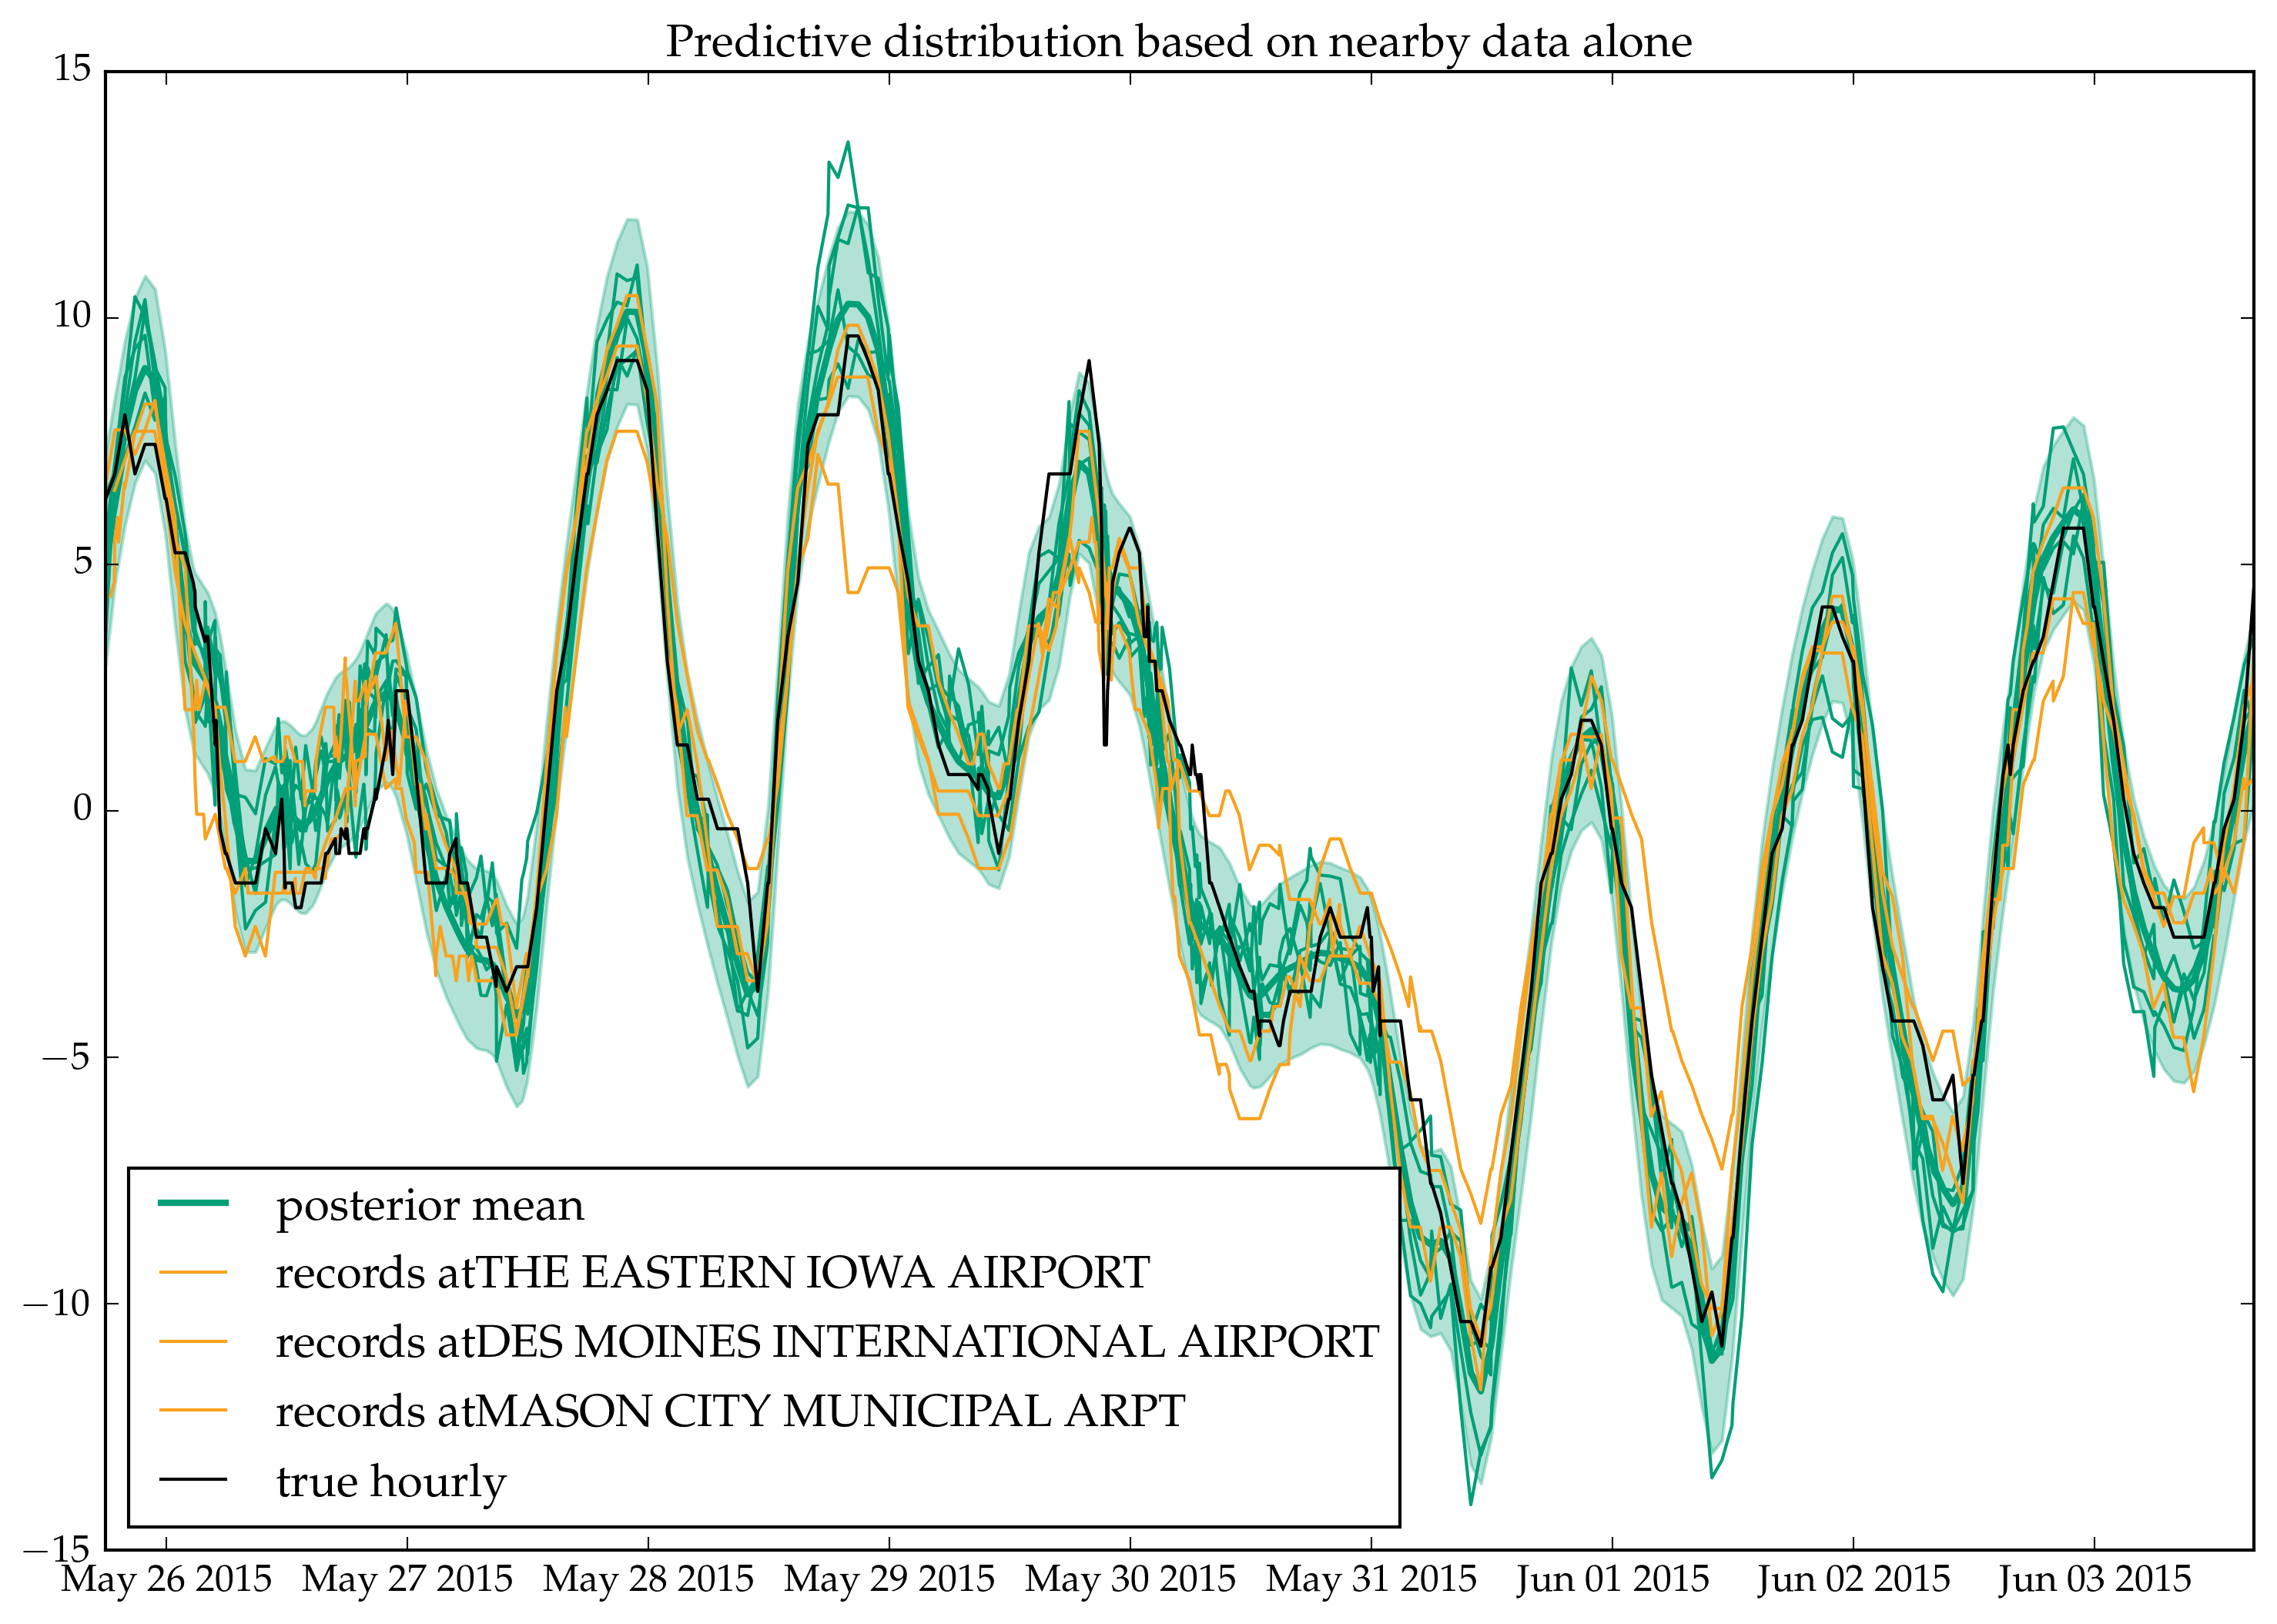
\includegraphics{figures/predictive_nearby_SEonly.png}
\caption{Predictive distribution using only nearby data and the simple
product of square exponentials model. The orange lines are the
measurements at nearby stations that are being used to inform the
predictions. The black line is the true temperatures that have been
withheld from the model, while the green line is the posterior mean of
the predictions. The credible range (in green) is twice the standard
deviations extracted from the diagonal entries of the posterior
covariance matrix.}
\end{figure}

Once we have a spatio-temporal Gaussian process model with optimized
covariance parameters, we can use it to generate predictions at the
station where we aim to generate imputations based on nearby
measurements. Gaussian processes make this a straightforward analytical
procedure. We'll denote the temperatures we wish to impute as
\(T_\miss{}\) at times \(t_\miss\) and location \(\xvec_\miss\) and
those observed at nearby stations as \(T_\obs{}\), at times \(t_\obs\)
and locations \(X_\obs\). Under the spatio-temporal model, \(T_\miss\)
and \(T_\obs\) are jointly multivariate normal, with mean zero and
covariance given by \(k_{st}(\xvec,\xvec',t,t')\). Standard results for
conditioning within multivariate normals then yields

\begin{align}
    T_\miss \mid T_\obs &\sim \normal\del{\mu_{\miss \mid \obs}, \Sigma_{\miss \mid \obs}}\,, \\
    \mu_{\miss \mid \obs} &= \cov\del{T_\miss, T_\obs} \cov\del{T_\obs, T_\obs}^{-1} T_\obs\,, \\
    \Sigma_{\miss \mid \obs} &= \cov\del{T_\miss,T_\miss} - \cov\del{T_\miss, T_\obs} \cov\del{T_\obs, T_\obs}^{-1} \cov\del{T_\obs, T_\miss}\,. \\ %_
\end{align}

All covariance matrices can be obtained by plugging into \(k_{st}\). For
example, the \(ij\)th entry of \(\cov\del{T_\miss, T_\obs}\) is given by
\(k_{st}(\xvec_\miss,X_\obs\sbr{j},t_\miss\sbr{i},t_\obs\sbr{j})\),
where \(X_\obs\sbr{j}\) gives the spatial covariates of the \(j\)th
observation, and \(t_\obs\sbr{j}\) its time.

In Figure X, we show an example of predictions obtained from this
spatio-temporal model. We witheld measurements from the Waterloo
Municipal Airport, and then used data from three nearby stations between
May 25, 2015 and June 3, 2015 to predict the Waterloo temperatures
during the same time window. This setup allows us to gauge the quality
of the predictions.
    


    	Our aim, however, isn't just to predict temperatures at a location with
no measurements, but rather to impute hourly temperatures at a location
with accurate measurements of the daily temperature extremes. Those
measurements can be thought of as constraints on the predictions. A
\(\Tx\) record means that in the 24 hours before the measurements, the
temperature reached \(\Tx\) but never exceeded it. Conceptually, we
could therefore implement a valid imputation algorithm by drawing random
samples from the posterior predictive multivariate normal distribution
obtained from nearby measurements, and only keeping the samples that
satisfy this constraint. Unfortunately, the probability of a random draw
exactly satisfying such a constraint is zero, and so there would need to
be some tolerance for overshooting or undershooting each day's \(\Tn\)
and \(\Tx\) constraints. Imputing longer periods would then require
either increasing the number of samples exponentially, or further
loosening this tolerance. Ultimately, this rejection sampling strategy
is therefore bound to fail.

Instead, we used the probabilistic programming language Stan to draw
samples from the constrained predictive distribution. In Stan, we
specify a probabilistic data-generating process for the observed
temperatures, based on parameters and latent variables with accompanying
priors. Stan then uses a Hamiltonian Monte Carlo (HMC) algorithm to draw
sample from the posterior distribution for the parameters and latent
variables. In our case, the observations are the daily maxima and
minima, the only parameter is the average temperature at the station of
interest \(\mu_\miss\), and the latent variables are the missing
unobserved hourly temperatures \(T_\miss\).

{[}Serious notation problems here:{]}

\begin{align}
    \mu_\miss &\sim \normal\del{0,100} \\
    f_\miss &\sim \normal\del{\mu_{\miss \mid \obs}, \Sigma_{\miss \mid \obs}} \\
    T_\miss &\sim \mu_\miss + f_\miss \\
    \Tx\sbr{d} &= \max\cbr{ T_{\miss,i}: t_{miss,i} \in d } \\
    \Tn\sbr{d} &= \min\cbr{ T_{\miss,i}: t_{miss,i} \in d } \\
\end{align}

The problem lies in the sharpness of the \(\max\) and \(\min\)
functions. At each step of the markov chain, a proposal is made for
\(T_\miss\). If the daily maxima and minima of this proposal coincide
exactly with the measurements, then its posterior probability is finite.
Otherwise it is exactly zero, with gradient also zero. HMC works by
exploiting the gradient of the posterior, and therefore fails to
converge in this situation, for reasons similar to the failure of the
naive rejection sampler.

We can rescue the algorithm by replacing the \(\max\) and \(\min\)
functions with the \(\softmax\) and \(\softmin\) functions, which take
real inputs \(x_1, \ldots, x_p\) and a sharpness parameter \(k\) and
return

\begin{align}
    \softmax\del{x_1, \ldots, x_p ; k} &= \log\del{\sum_{i=1}^p e^{kx_i}} \\
    \softmin\del{x_1, \ldots, x_p ; k} &= -\softmax\del{-x_1, \ldots, -x_p; k}
\end{align}

As \(k \rightarrow \infty\), \(\softmax\) becomes the maximum, and
\(\softmin\) becomes the minimum. Lower values of \(k\) give close
approximations. When \(\softmax\) replaces \(\max\) and \(\softmin\)
replaces \(\min\), there is a small price in precision due to the
approximation, but there is a huge computational benefit. Gradients are
now available, and the posterior doesn't go abruptly to zero when the
conditions aren't met exactly. This in turns makes HMC a viable
algorithm to efficiently draw samples from the posterior. Setting \(k\)
is a compromise between exactness and efficiency; we found \(k=10\) to
perform well.

\begin{figure}
\centering
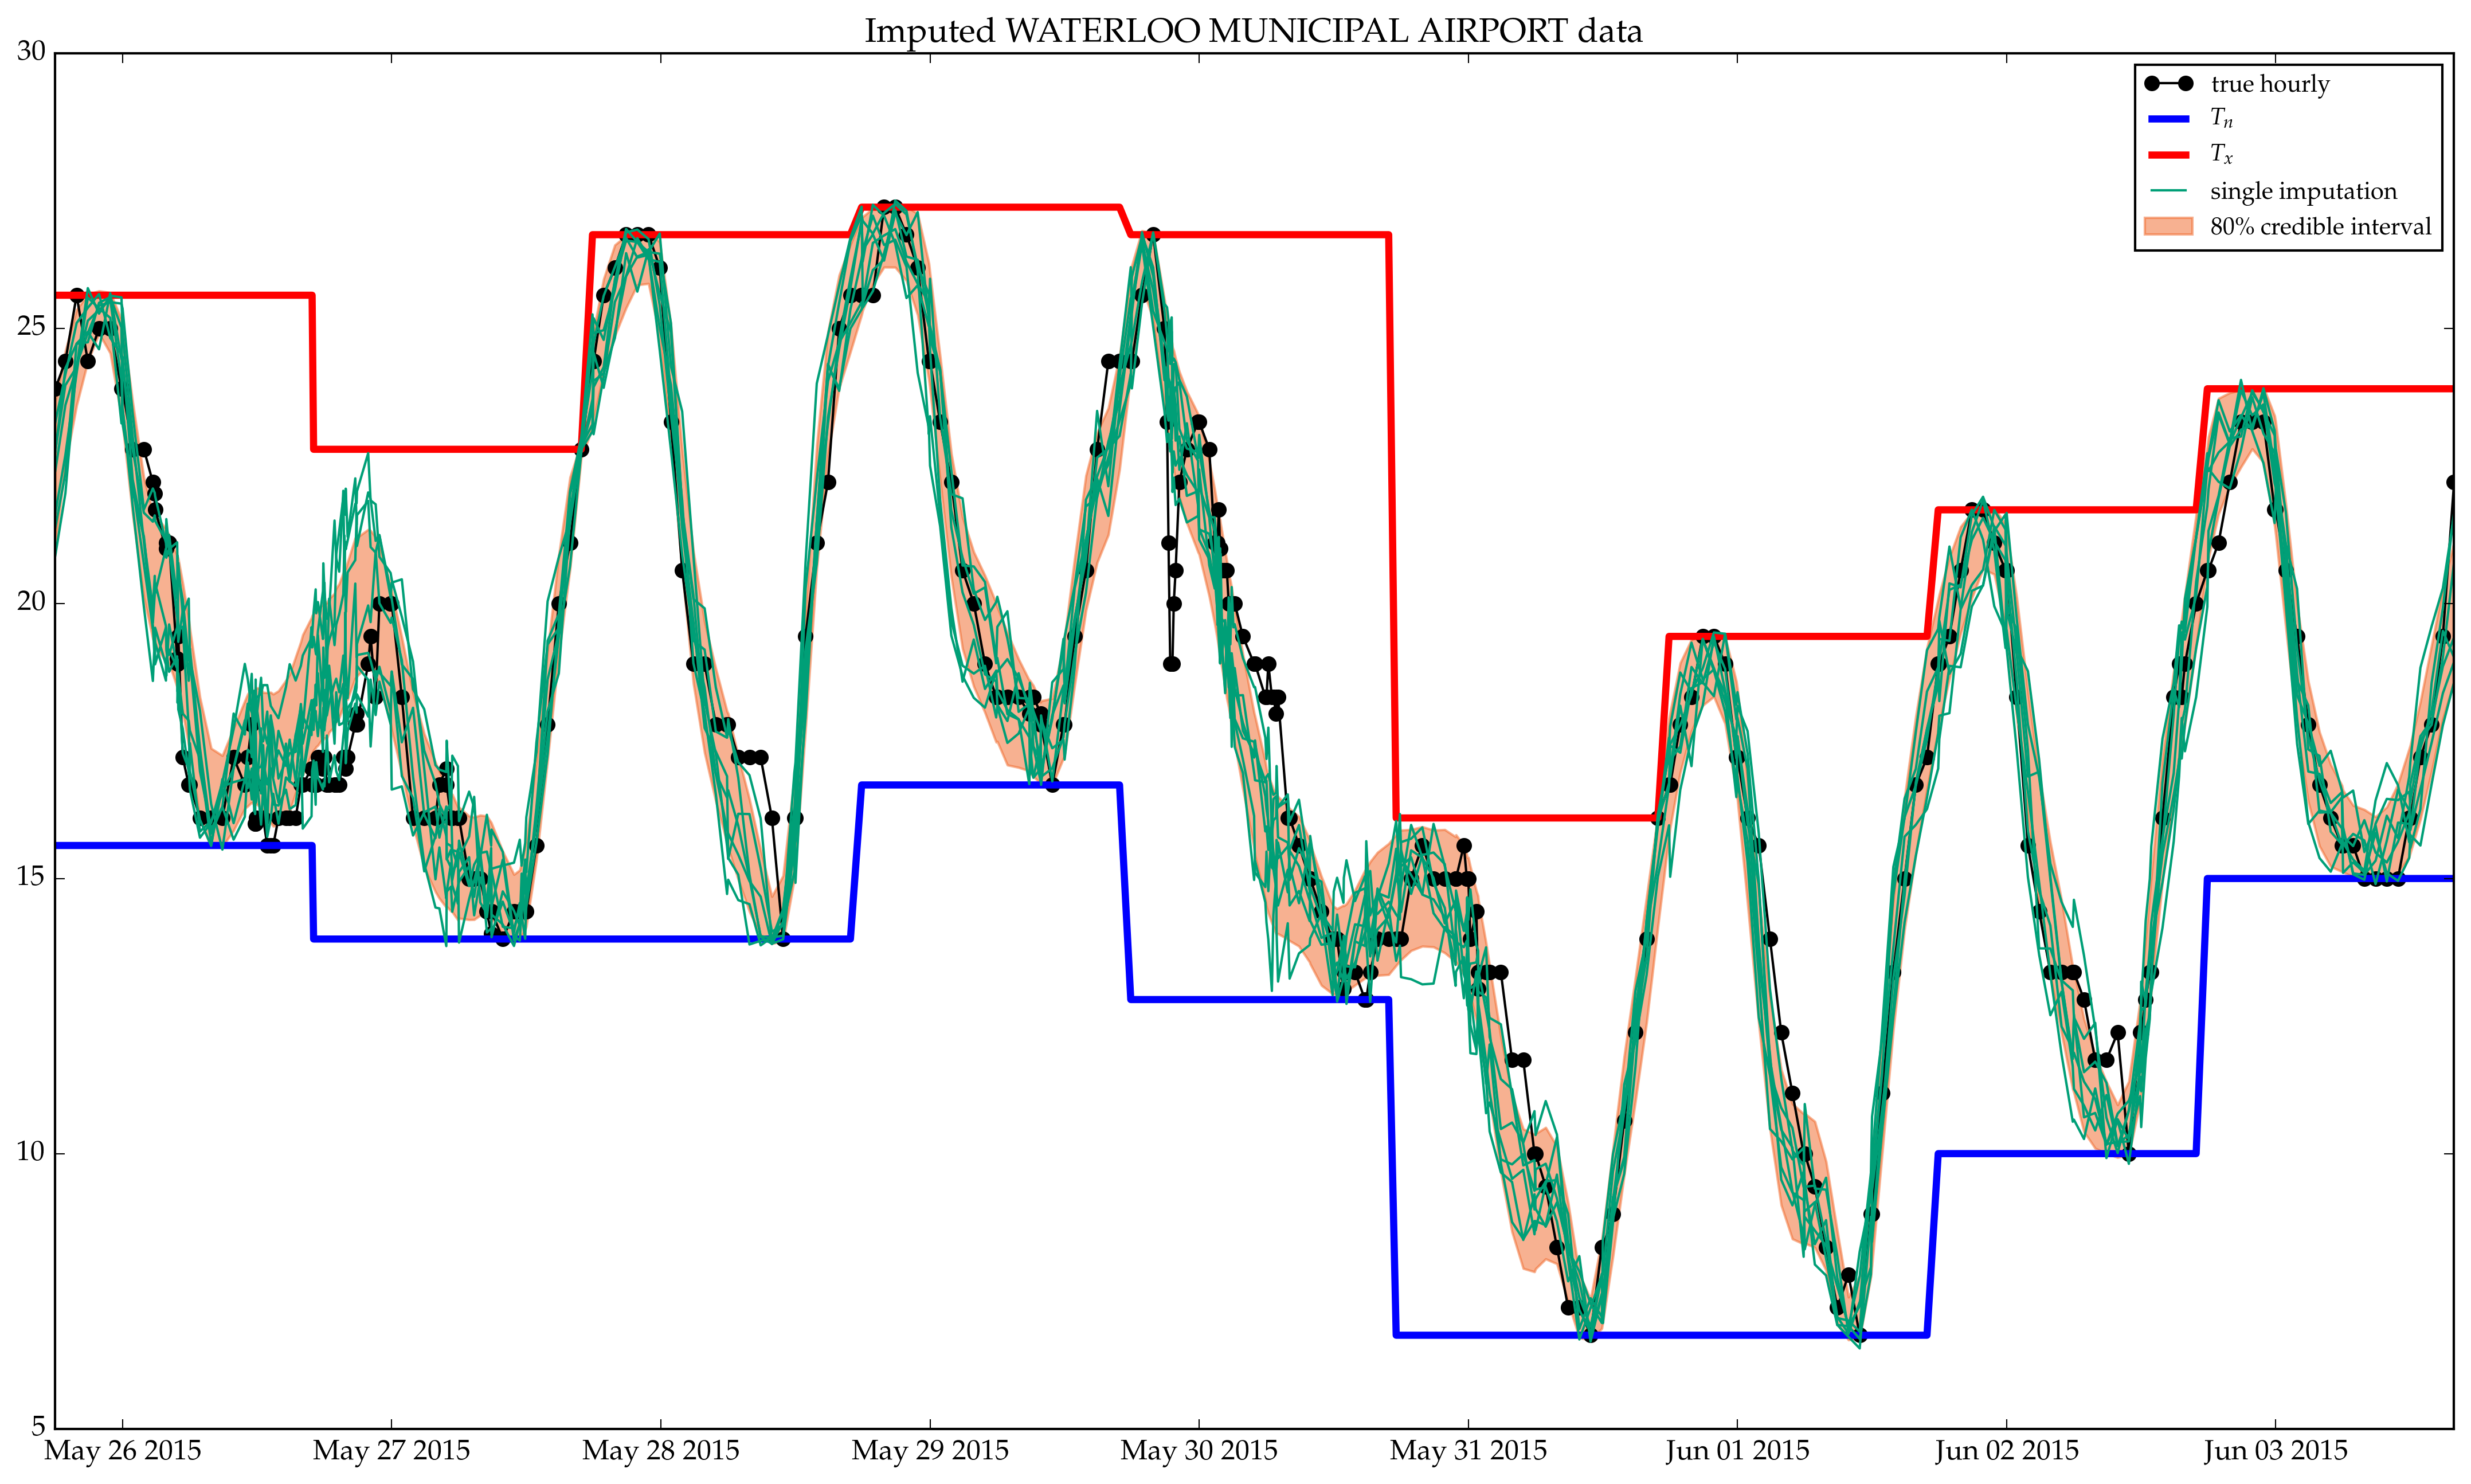
\includegraphics{figures/imputations_SEonly.png}
\caption{Imputations at Waterloo Airport from May 25, 2015 to June 3,
2015}
\end{figure}

One additional modification was necessary because of a quirk in the Stan
modeling language. The observations have to be drawn from a random
distribution, and so we added some Gaussian noise with a small standard
deviation. The full model we implemented is below, and is an
approximation of our ideal model above.

\begin{align}
    \mu_\miss &\sim \normal\del{0,100} \\
    f_\miss &\sim \normal\del{\mu_{\miss \mid \obs}, \Sigma_{\miss \mid \obs}} \\
    T_\miss &\sim \mu_\miss + f_\miss \\
    \Tx\sbr{d} &\sim \normal\del{\softmax\cbr{ T_{\miss,i}: t_{miss,i} \in d; k=10}, 0.1} \\
    \Tn\sbr{d} &\sim \normal\del{\softmax\cbr{ T_{\miss,i}: t_{miss,i} \in d; k=10}, 0.1} \\
\end{align}

Example imputations from this procedure are shown in Figure X. From May
25, 2015 to June 3, 2015, hourly temperatures are imputed at Waterloo
Airport, using the hourly temperature measurements from nearby stations
to inform the course of the temperatures, and using the daily minima and
maxima ``measurements'' to constrain the imputed temperatures, and to
infer the mean. Because we actually have hourly data for Waterloo, yet
only fed our algorithm a reduction of this data to daily extremes, we
can also plot the hidden temperatures, and see how faithfully the
imputations reproduce them. We see that the imputations indeed track the
truth very closely. The error bars satisfyingly narrow and widen in
accordance to the amount of information available at each moments. On
May 27th, we can see that the imputations capture the fact that the
\(\Tx\) record \emph{could} have been set early in the measurement
window, but more likely at its very end.
    


    	\section{Model diagnostic}\label{model-diagnostic}
    


    	\section{Improving model}\label{improving-model}

\begin{enumerate}
\def\labelenumi{\arabic{enumi}.}
\tightlist
\item
  focused on timeseries model

  \begin{itemize}
  \tightlist
  \item
    kernel components
  \item
    diurnal cycle
  \item
    show improved variograms
  \end{itemize}
\item
  spatiotemporal model

  \begin{itemize}
  \tightlist
  \item
    variograms and cross-variograms
  \item
    trace evolution

    \begin{itemize}
    \tightlist
    \item
      product kernel
    \item
      sum of products with variance 1
    \item
      sum of products with free variance
    \end{itemize}
  \item
    for each model, report marginal likelihood, and predictive
    diagnostic in a table
  \item
    discuss importance of getting uncertainty right
  \end{itemize}
\end{enumerate}

\section{Analysis}\label{analysis}

\begin{itemize}
\tightlist
\item
  show imputations on interesting days
\item
  show imputations can capture two possible explanations for a
  measurement
\item
  discuss possibility of inferring measurement time
\end{itemize}
    



    % Add a bibliography block to the postdoc
    
    
    
    \end{document}
